\documentclass[UTF8]{ctexart}
%这里是导言区
\title{毕业设计资料}
\author{Kangkang}
\date{\today}
\usepackage{xeCJK}
\usepackage{graphicx}
\usepackage{pythonhighlight}
\setCJKmainfont{楷体}
\usepackage{amsmath}
\graphicspath{{C:/Users/KangKang/Desktop/Graduation-Project/demo/Graphs/}}
\begin{document}
\maketitle
\section{Dataset}
\subsection{来源}
https://physionet.org/physiobank/database/noneeg/

Reference:
Birjandtalab, Javad, Diana Cogan, Maziyar Baran Pouyan, and Mehrdad Nourani, A Non-EEG Biosignals Dataset for Assessment and Visualization of Neurological Status, 2016 IEEE International Workshop on Signal Processing Systems (SiPS), Dallas, TX, 2016, pp. 110-114. doi: 10.1109/SiPS.2016.27
\subsection{描述}
用于推断20名健康人的神经状态(包括身体压力,认知压力,情绪压力和放松)。

使用非侵入式手腕佩戴的生物传感器收集数据,并且包括电活动(EDA),温度,加速度,心率(HR)和动脉血氧饱和度(SpO2)。

数据包括20个样本的7个阶段数据:
\begin{enumerate}
\item 放松5min
\item 身体压力:站立1min,以每小时一英里的速度步行2min,然后在跑步机上以每小时三英里的速度步行/慢跑2min
\item 放松5min
\item 小情绪压力:40s,告知被试在接下来的3min会计算从2485每次减7的结果(注意:这部分数据是在认知压力任务之前收集的,在本文中没有解释)
\item 认知压力:计算3min,进行Stroop测试2min。Stroop测试:读取用不同颜色墨水的笔写的颜色名称,说出墨水的颜色
\item 放松5min
\item 情绪压力:告知志愿者会在1min内从一部恐怖电影中看到一个5min的片段。 经过一段时间后,播放《部落》的片段
\item 放松5min
(我们本来并不打算把指令的读数算作情绪压力。 毕竟,每个任务都有指示。 然而,与其他指令集不同的是,这一项在许多志愿者身上产生了压力反应,这对测试管理员来说是显而易见的。)
\end{enumerate}
数据文件以WFDB格式提供,每个被试有两个record:一个包含加速度,温度和EDA信号,另一个包含SpO2和心率信号。.hea文件包含有关该被试的信息。每个记录有一个注释文件,用于指示转换状态的时间位置和标签。subjectinfo.csv文件还包含有关每个主题的信息。

\subsection{数据读取}
每个被试的数据包括以下五个文件:
\begin{itemize}
\item Subject * \_AccTempEDA.atr
\item Subject * \_AccTempEDA.dat
\item Subject * \_AccTempEDA.hea
\item Subject * \_SpO2HR.dat
\item Subject * \_SpO2HR.hea
\end{itemize}


其中*表示$1 \sim 20$.
\subsubsection{读取$AccTempEDA.atr$文件}
.atr文件为ATE信号文件的注释文件,指示转换状态的时间位置和标签。使用WFDB包中的rdann函数进行读取。
\newtheorem{thm}{Function}
\begin{thm}
annotation = rdann(recordname, extension, sampfrom=0, sampto=None, shiftsamps=False,
pbdir=None, return\_label\_elements=['symbol'], summarize\_labels=False)
\end{thm}
\begin{python}
import wfdb
ann = wfdb.rdann('C:/Users/KangKang/Desktop/Graduation-Project/Dataset/Subject1_AccTempEDA', 'atr')
\end{python}
ann中包含以下参数,可以通过$ann.\_$调用.
\begin{tabbing}
\textbf{extension}\quad\quad\quad\quad\quad\quad\= 所处文件扩展名\\[5pt]
\textbf{sample}											\> 标记所处的位置\\[5pt]
\textbf{symbol}											\> 用于标记的符号\\[5pt]
\textbf{subtype}										\> 标记的类型\\[5pt]
\textbf{chan}											\> 标记所处的通道\\[5pt]
\textbf{num}												\> 每种标记的数目\\[5pt]
\textbf{aux\_note}										\> 标记的辅助信息\\[5pt]
\textbf{fs}												\> 每条记录的采样频率\\[5pt]
\textbf{label\_store}									\> 用于存储/编码每个注释标签的整数值\\[5pt]
\textbf{description}									\> 每个注释标签的描述性字符串\\[5pt]
\textbf{custom\_labels}								\> 注释文件中定义的自定义注释标签\\[5pt]
\textbf{contained\_labels}							\> 此注释中包含的唯一标签\\
\end{tabbing}
查看ann的参数,发现在该数据库中有用的参数有以下几个:
\begin{center} 
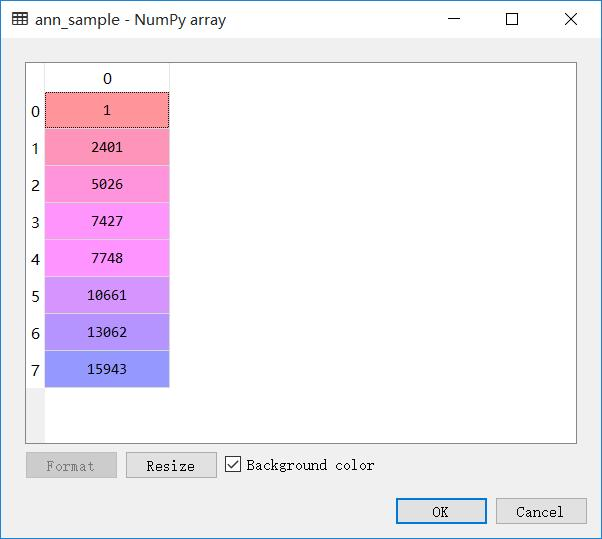
\includegraphics[angle=0,width=0.8\textwidth]{ann_sample.jpg}\\
\vspace{3mm}
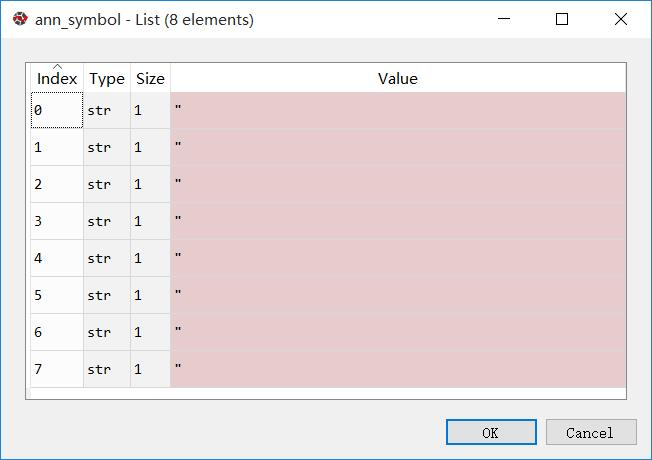
\includegraphics[angle=0,width=0.8\textwidth]{ann_symbol.jpg}\\
\vspace{3mm}
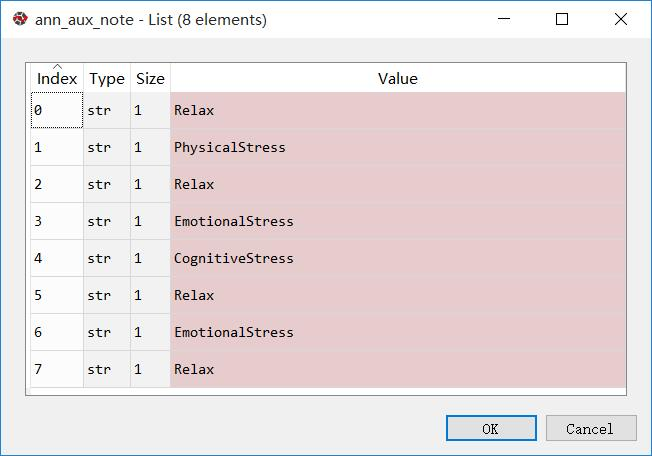
\includegraphics[angle=0,width=0.8\textwidth]{ann_aux_note.jpg}\\ 
\end{center}
其中$ann.sample$记录标记所在的点的位置,$ann.symbol$表明该数据库中的标记用'\''表示,$ann.aux\_note$表示标记的含义分别为:Relax-PhysicalStress-Relax-EmotionalStress-ConitiveStress-Relax-EmotionalStress-Relax.
\subsubsection{读取$AccTempEDA.dat$文件和$AccTempEDA.hea$}
.dat文件为ATE信号文件的数据文件,.hea为ATE信号的头文件。使用WFDB包中的rdsamp函数进行读取。
\begin{thm}
record = rdsamp(recordname, sampfrom=0, sampto=None, channels=None,
physical=True, pbdir = None, m2s=True)
\end{thm}
\begin{python}
import wfdb
ATE_dat = wfdb.rdsamp(root+'Subject2_AccTempEDA')
\end{python}
ATE\_dat中包含以下参数,可以通过$ATE\_dat.\_$调用.
\begin{tabbing}
\textbf{p\_signals}\quad\quad\quad\quad\quad\quad\= 五个通道的数据\\[5pt]
\textbf{fs}											\> 采样频率\\[5pt]
\textbf{units}											\> 单位\\[5pt]
\textbf{signame}										\> 信号的名字\\[5pt]
\textbf{comments}											\> 其他信息\\
\end{tabbing}
查看ATE\_dat的参数,发现在该数据库中有用的参数有以下几个:
\begin{center} 
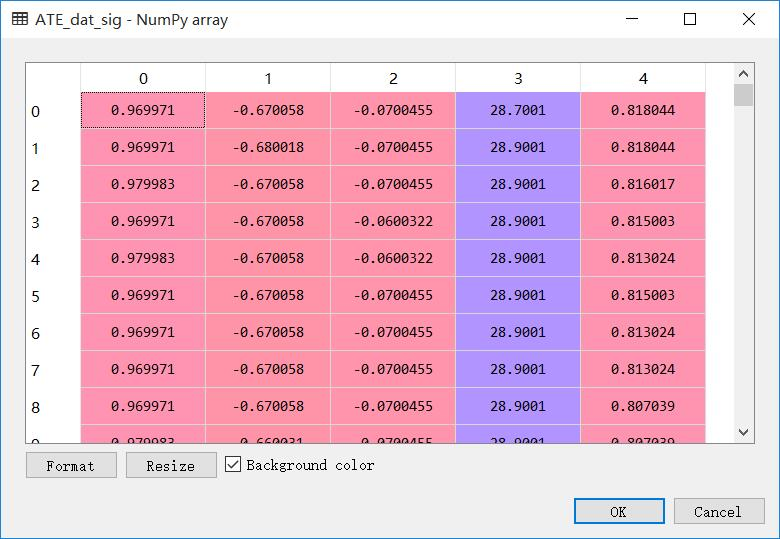
\includegraphics[angle=0,width=0.8\textwidth]{ATE_dat_sig.jpg}\\
\vspace{3mm}
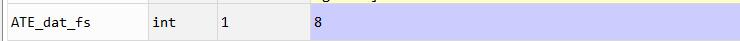
\includegraphics[angle=0,width=0.8\textwidth]{ATE_dat_fs.jpg}\\
\vspace{3mm}
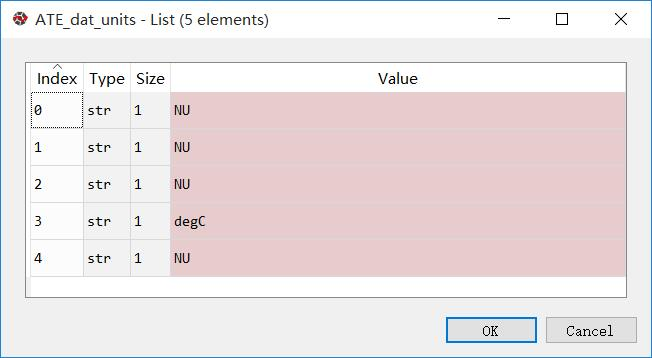
\includegraphics[angle=0,width=0.8\textwidth]{ATE_dat_units.jpg}\\
\vspace{3mm}
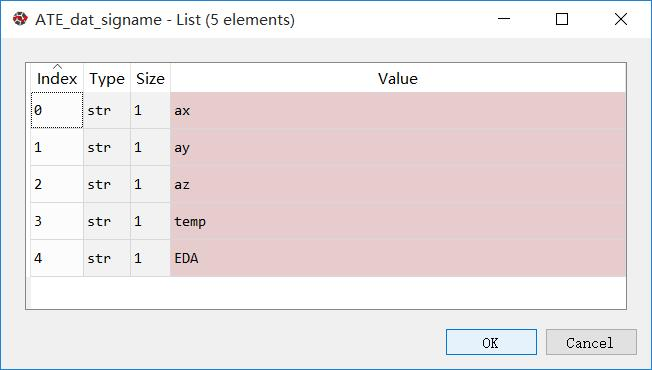
\includegraphics[angle=0,width=0.8\textwidth]{ATE_dat_signame.jpg}\\
\vspace{3mm}
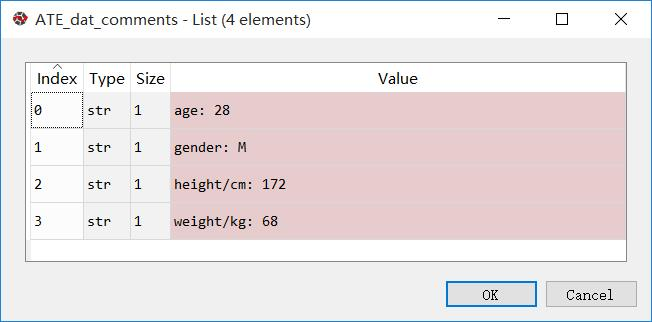
\includegraphics[angle=0,width=0.8\textwidth]{ATE_dat_comments.jpg}\\ 
\end{center}
其中$ATE\_dat.p\_signals$记录五个通道的数据:三轴加速度、温度、EDA,$ATE\_dat.fs$记录采样率,为8Hz,$ATE\_dat.units$记录单位,分别为:nv, nv, nv, degC, nv,$ATE\_dat.signame$记录信号的名称,分别为:ax, ay, az, Temp, EDA,$ATE\_dat.comments$记录其他信息,包括:年龄、性别、身高、体重。

使用自带的作图包绘图,结果如下:
\begin{center} 
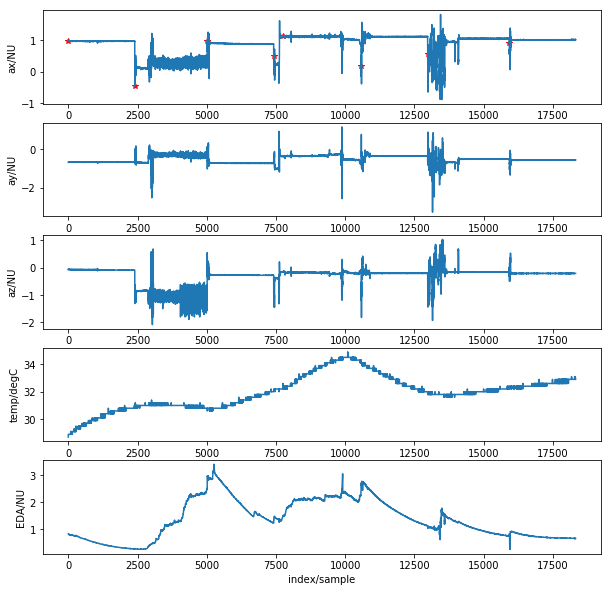
\includegraphics[angle=0,width=0.8\textwidth]{fig1.png}\\
\end{center}
\subsubsection{读取$SpO2HR.dat$文件和$SpO2HR.hea$}
.dat文件为SH信号文件的数据文件,.hea为SH信号的头文件。使用WFDB包中的rdsamp函数进行读取。
\begin{thm}
record = rdsamp(recordname, sampfrom=0, sampto=None, channels=None,
physical=True, pbdir = None, m2s=True)
\end{thm}
\begin{python}
import wfdb
SH\_dat = wfdb.rdsamp(root+'Subject2_SpO2HR')
\end{python}
SH\_dat中包含以下参数,可以通过$SH\_dat.\_$调用.
\begin{tabbing}
\textbf{p\_signals}\quad\quad\quad\quad\quad\quad\= 两个通道的数据\\[5pt]
\textbf{fs}											\> 采样频率\\[5pt]
\textbf{units}											\> 单位\\[5pt]
\textbf{signame}										\> 信号的名字\\[5pt]
\textbf{comments}											\> 其他信息\\
\end{tabbing}
查看ATE\_dat的参数,发现在该数据库中有用的参数有以下几个:
\begin{center} 
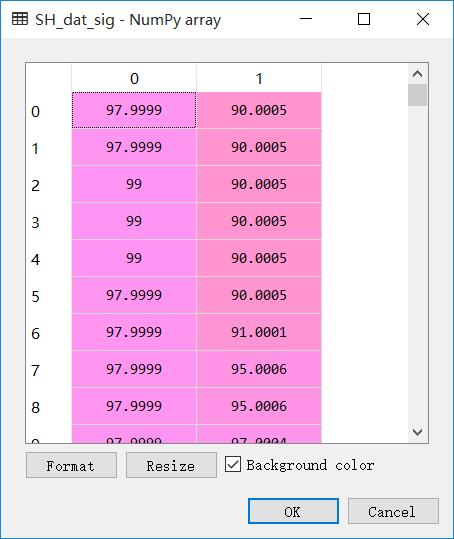
\includegraphics[angle=0,width=0.8\textwidth]{SH_dat_sig.jpg}\\
\vspace{3mm}
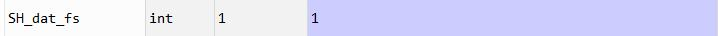
\includegraphics[angle=0,width=0.8\textwidth]{SH_dat_fs.jpg}\\
\vspace{3mm}
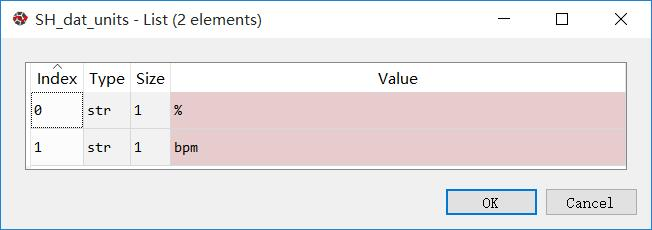
\includegraphics[angle=0,width=0.8\textwidth]{SH_dat_units.jpg}\\
\vspace{3mm}
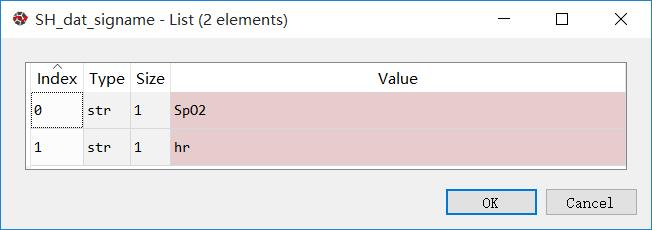
\includegraphics[angle=0,width=0.8\textwidth]{SH_dat_signame.jpg}\\
\vspace{3mm}
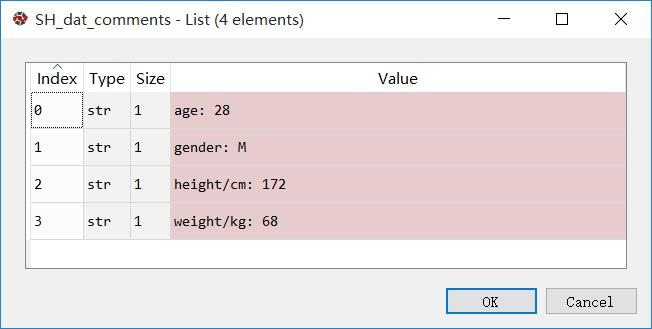
\includegraphics[angle=0,width=0.8\textwidth]{SH_dat_comments.jpg}\\ 
\end{center}
其中$SH\_dat.p\_signals$记录两个通道的数据:血氧饱和度,心率,$SH\_dat.fs$记录采样率,为1Hz,$SH\_dat.units$记录单位,分别为:\%、bpm,$SH\_dat.signame$记录信号的名称,分别为:SpO2,hr,$SH\_dat.comments$记录其他信息,包括:年龄、性别、身高、体重。

使用自带的作图包绘图,结果如下:
\begin{center} 
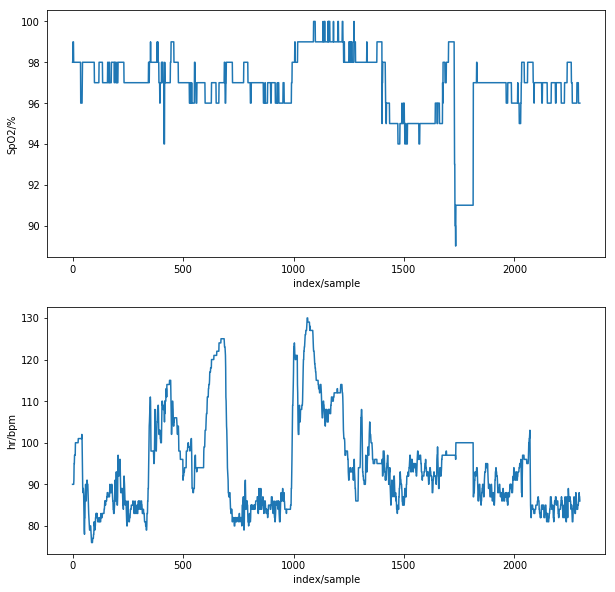
\includegraphics[angle=0,width=0.8\textwidth]{fig2.png}\\
\end{center}
\end{document}